\documentclass[tikz,border=10pt]{standalone}
% Scale: s = 0.009963 cm/px, centred on the rectangle; y flipped.
\begin{document}
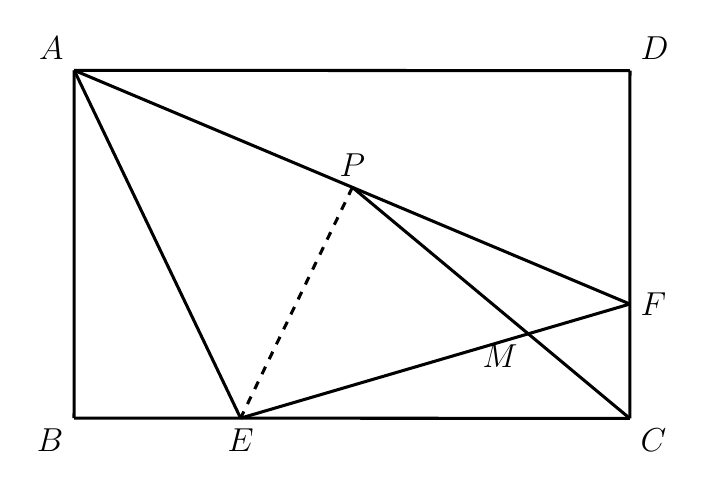
\begin{tikzpicture}[line width=1.1pt, line join=round]
  % Named coordinates (cm)
  \coordinate (A) at (-3.5285448127561985,2.2098731296364096);
  \coordinate (D) at (3.5295689387225595,2.2058744490789506);
  \coordinate (C) at (3.5270670363847723,-2.210260083662475);
  \coordinate (B) at (-3.5310467150939857,-2.2062614031050156);
  \coordinate (E) at (-1.4152775245536449,-2.2074600640255078);
  \coordinate (F) at (3.5278896963184323,-0.7581742500664895);
  \coordinate (P) at (0.004511351137426178,0.7238141183748139);
  \coordinate (M) at (2.2378320298406384,-1.136405896230686);

  % Rectangle ABCD
  \draw (A) -- (B);
  \draw (B) -- (C);
  \draw (C) -- (D);
  \draw (D) -- (A);

  % Segments
  \draw (A) -- (F);      % passes through P
  \draw (A) -- (E);
  \draw (E) -- (F);
  \draw (P) -- (C);

  % Dashed segment
  \draw[dashed] (P) -- (E);

  % Labels
  \node[font=\fontsize{11.5}{13.8}\selectfont, above left]  at (A) {$A$};
  \node[font=\fontsize{11.5}{13.8}\selectfont, above right] at (D) {$D$};
  \node[font=\fontsize{11.5}{13.8}\selectfont, below left]  at (B) {$B$};
  \node[font=\fontsize{11.5}{13.8}\selectfont, below right] at (C) {$C$};
  \node[font=\fontsize{11.5}{13.8}\selectfont, below]       at (E) {$E$};
  \node[font=\fontsize{11.5}{13.8}\selectfont, right]       at (F) {$F$};
  \node[font=\fontsize{11.5}{13.8}\selectfont, above]       at (P) {$P$};
  \node[font=\fontsize{11.5}{13.8}\selectfont, below left]  at (M) {$M$};
\end{tikzpicture}
\end{document}
% GEOAGENT_REPAIR_V1 c18a466396f54661 5e25c4f835999b3f36ccafbdc195030686fdfdd07ff872ba6016fb1abdbaad01
